%%%%%%%%%%%%%%%%%%%%%%%%%%%%%%
%
% Physics Lab Report #1
% Ver 1
% 09.01.2017
% Author: Abdollah Shajadi
% Teacher: Susanna Kujanpää
% 
%  OAMK | DIN16SP 
%
%%%%%%%%%%%%%%%%%%%%%%%%%%%%%%

%------------------------------
% Packages and configurations
%------------------------------

\documentclass[a4paper, 12pt]{article}
\usepackage[T1]{fontenc}
\usepackage[utf8]{inputenc}
\usepackage[a4paper, top=1.6in, bottom=1.6in, left=1in, right=1in]{geometry}
\usepackage{fancyhdr}
\pagestyle{fancy}
\fancyhf{}
\renewcommand{\headrulewidth}{0pt}
\renewcommand{\footrulewidth}{0pt}
\fancyhead[L]{}
\fancyhead[R]{
	
\includegraphics[width=3cm]{oamk.jpg}
}
\rfoot{\thepage}
\usepackage[protrusion=true,expansion=true]{microtype}
\usepackage{graphicx}
\usepackage{caption}
\usepackage{subcaption}
\usepackage{amsmath}
\usepackage{amssymb}
\usepackage{siunitx}
\usepackage{mathpazo}
\linespread{1.05}
\makeatletter
\renewcommand\@biblabel[1]{\textbf{#1.}}
\renewcommand{\@listI}{\itemsep=0pt}

\renewcommand{\maketitle}{ 
	\begin{flushright} 

		{\LARGE\@title} 
		
		\vspace{80pt} 
		
		{\large\@author} 
		
		\vspace{170pt} 
	\end{flushright}
}

%------------------------------
%  Title 
%------------------------------
\vspace*{\fill}
\title{\textbf{Physics Lab Report Work 1}\\
	Determination of the density of the body} 

\author{\textsc{Author: Abdollah Shajadi}
	\\{\textsc{Teacher: Susanna Kujanp{\"a}{\"a}}}
	\\{\textsc{Team members: Abdollah Shajadi, Yulia Yuvminina}}
	\\{\textsc{Date of work: 27.01.2017}}
	\\{\textsc{Date of return: 10.02.2017}}
	\\{\textsc{DIN16SP}}}

\begin{document}
	
	\maketitle 
	
\clearpage

\tableofcontents

\clearpage
%------------------------------
%  Summary and Keywords 
%------------------------------

\renewcommand{\abstractname}{Summary} 

\begin{abstract}

In this Lab work we measure and determine the density of rectangular parallelogram and cylinder.
we will measure the weight of parallelogram and cylinder with balance scale in air and then only parallelogram also in water and unknown liquid (alcohol), with 10 time measurements of diameter of the base and the height for cylinder and 3 sides of parallelogram we calculate the density. 
In the following pages comes the theory, calculations, formulas and the measures.

\end{abstract}

\hspace*{3,6mm}\textit{Keywords:} Density, Measurements, Micrometer, Caliper, Error estimation 

\vspace{30pt}

%------------------------------
%	Body
%------------------------------

\section{Theory}

Density (\(\rho\)) is defined by following equation where \(m\) is mass and \(v\) is volume of the body.

\[\rho = \frac{m}{v}\]

According to Archimedes' principle if the weight of the water displaced is less than the weight of the object, the object will sink, Otherwise the object will float, with the weight of the water displaced equal to the weight of the object. \cite{weber}
As described the buoyancy is equal to weight of displaced fluid in Archimedes' principle.

\[
\rho = \frac{m_{a}}{m_{a}-m_{w}}.\rho_{w}
\]

Where \(m_{a}\) is mass of the body that measured surrounded by air and \(m_{l}\) is mass of the body measured surrounded by liquid and \(\rho_{l}\) is density fo the liquid.

For Calculating density of rectangular parallelogram according to density formula and \(v=abc\) we get:

\[\rho = \frac{m_{1}}{abc} \]

And for the Cylinder we substitute \(v\) in density formula \(v = \frac{\pi d^{2} h}{4} \) .

%------------------------------

\section{Equipments}

We used a variety of different equipments, the following list is the main tools we used for the tasks.

\begin{figure}
	\centering
	\begin{minipage}{.5\textwidth}
		\centering
		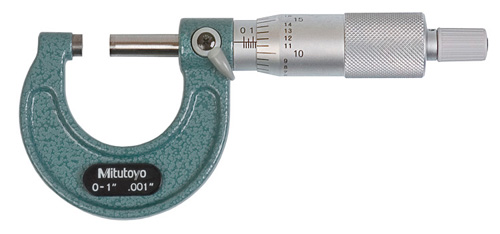
\includegraphics[width=.4\linewidth]{micrometer.jpg}
		\captionof{figure}{Micrometer}
	\end{minipage}%
	\begin{minipage}{.5\textwidth}
		\centering
		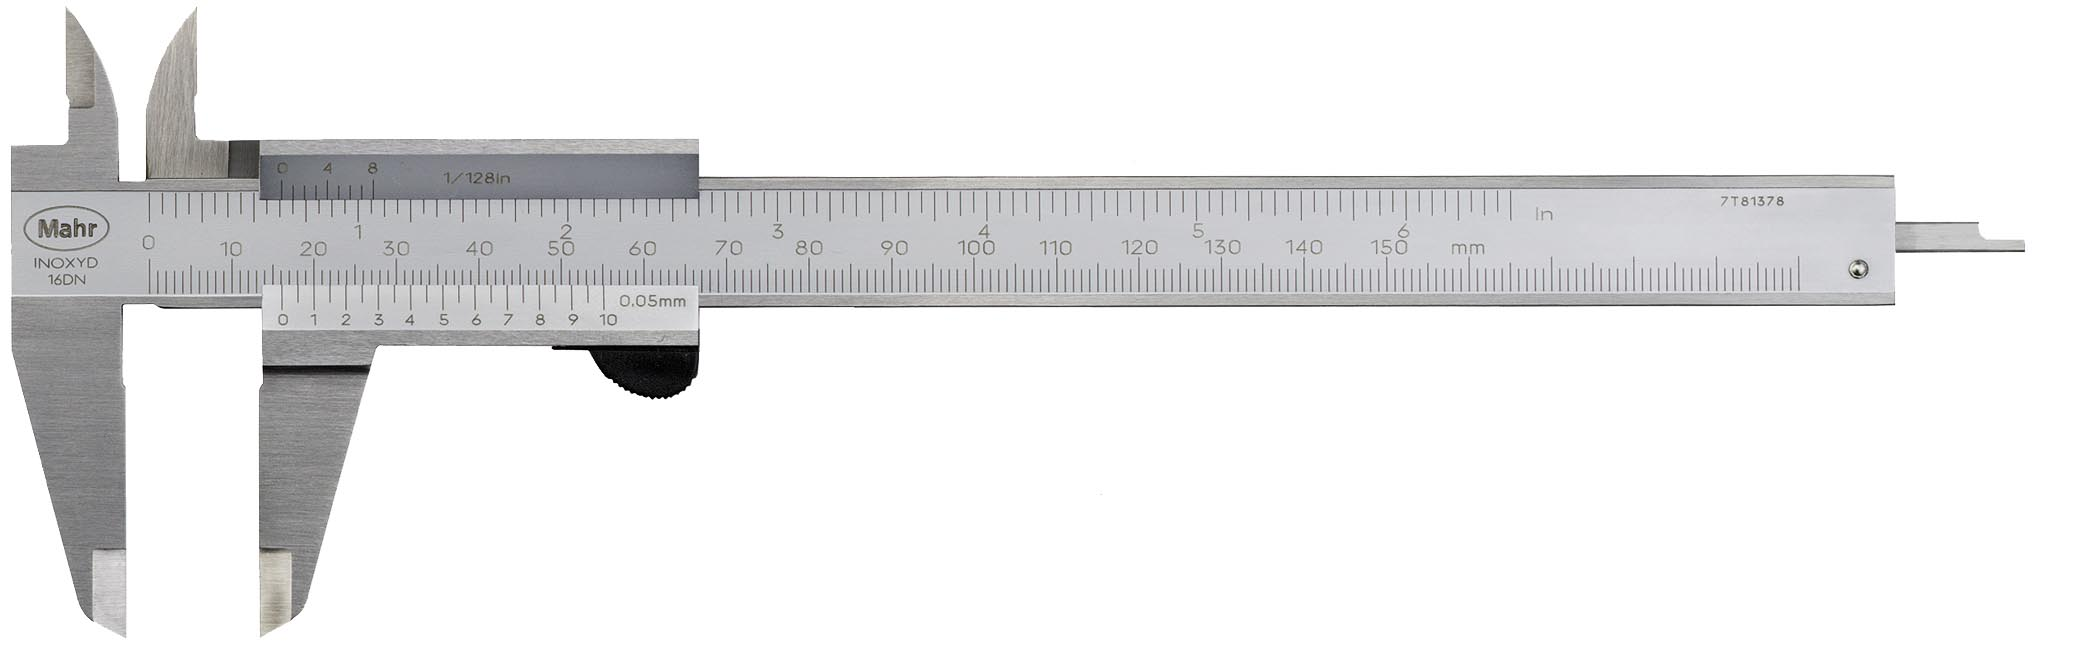
\includegraphics[width=.4\linewidth]{caliper.jpg}
		\captionof{figure}{Caliper}
	\end{minipage}
\end{figure}

\begin{enumerate}
	\item Micrometer (Figure 1)
	\item Caliper (Figure 2)
	\item Balance Scale
	\item Aerometer
	\item Water
	\item Alcohol (as unknown liquid)
	\item String
	\item Metal parallelogram
	\item Metal Cylinder
	\item Beaker
\end{enumerate}

%------------------------------
\section{Measurments and Calculations}

All the measurements and calculations are based on the work 1 formulas and instruction paper and signed result paper can be found on the last page of this report. on the following sections comes the detailed calculations of the lab.

\subsection{Density of rectangular parallelogram}

For the rectangular parallelogram we measured 3 sides of a, b and c for 10 times with Micrometer, following table shows the results of the measurements.

\begin{center}
	\begin{tabular}{||c c c c||} 
		\hline
		   &  a\((mm)\) & b\((mm)\)  &  c\((mm)\)  \\ [0.5ex] 
		\hline\hline
		1 & 20.00 & 20.01 & 14.40 \\ 
		\hline
		2 & 20.01 & 20.00 & 14.38 \\
		\hline
		3 & 20.00 & 20.00 & 14.45 \\
		\hline
		4 & 19.98 & 20.02 & 14.47 \\
		\hline
		5 & 20.00 & 20.01 & 14.44 \\
		\hline
		6 & 20.00 & 20.00 & 14.39 \\
		\hline
		7 & 20.02 & 19.99 & 14.39 \\
		\hline
		8 & 19.99 & 20.00 & 14.42 \\
		\hline
		9 & 20.00 & 19.98 & 14.49 \\
		\hline
		10 & 20.00 & 19.99 &  14.37 \\ [1ex] 
		\hline
	\end{tabular}
\end{center}

And using balance scale we got \(m_{1}\)= 43.90\(mm\) with the accuracy of \(\varDelta m\)= 0.01\(g\). and according to density formula we have:

\[
\rho = \frac{m}{v} = \frac{m}{abc} = \frac{43.90g}{20_{mm}.20_{mm}.14.42_{mm}} = \frac{43.90g}{5768_{mm^{3}}} \approx 7.611\times10^{-3}_{\frac{g}{mm^{3}}}
\]

Also we can calculate density with Archimedes’ principle for rectangular parallelogram based on our measurement for water and unknown liquid (Alcohol) that measured using aerometer:

\[
\rho = \frac{m_{a}}{m_{a}-m_{w}}.\rho_{w} = \frac{43.90g}{43.90_{g} - 38.20_{g}} \times 0.0010_{\frac{g}{mm^{3}}} \approx 7.702\times10^{-3}_{\frac{g}{mm^{3}}}
\]


\subsection{Density of Alcohol (unknown liquid)}

We can calculate density of unknown liquid (Alcohol) with Archimedes’ principle equation and with the help of known mass of rectangular parallelogram as follow:

We derive the following equation: \(\rho_{u} = \frac{m_{a}-m_{u}}{m_{a}} . \rho \), and we calculate it twice with our \(\rho\) of parallelogram form water and air. 


\[\rho_{u_{1}} = \frac{43.90_{g} - 39.45_{g} }{43.90{g}} \times 7.611\times10^{-3}_{\frac{g}{mm^{3}}} \approx  7.715\times10^{-4}_{\frac{g}{mm^{3}}} \]

\[\rho_{u_{2}} = \frac{43.90_{g} - 39.45_{g} }{43.90{g}} \times 7.702\times10^{-3}_{\frac{g}{mm^{3}}} \approx 7.807\times10^{-4}_{\frac{g}{mm^{3}}} \]


And then we calculate the average:

\[\rho_{u_{av}} = \frac{7.715\times10^{-4}_{\frac{g}{mm^{3}}} + 7.807\times10^{-4}_{\frac{g}{mm^{3}}} }{2} \approx 7.761\times10^{-4}_{\frac{g}{mm^{3}}}  \]


\subsection{Density of cylinder}

We measured height and diameter with Caliper the following table shows the result of the measurements.

\begin{center}
	\begin{tabular}{||c c c||} 
		\hline
		&  h\((mm)\) & d\((mm)\)  \\ [0.5ex] 
		\hline\hline
		1 & 24.90 & 18.00 \\ 
		\hline
		2 & 24.70 & 17.95 \\
		\hline
		3 & 24.40 & 17.90 \\
		\hline
		4 & 24.30 & 18.10 \\
		\hline
		5 & 24.40 & 18.00 \\
		\hline
		6 & 24.60 & 17.95 \\
		\hline
		7 & 24.70 & 18.20 \\
		\hline
		8 & 24.70 & 18.10 \\
		\hline
		9 & 24.40 & 17.90  \\
		\hline
		10 & 24.50 & 18.00 \\ [1ex] 
		\hline
	\end{tabular}
\end{center}

Now with the help of Cylinder density formula and average of the \(h\) and \(d\) we have:

\[
\rho = \frac{m}{v} = \frac{m}{ \frac{\pi d^{2} h}{4}} = \frac{4m}{\pi d^{2} h} = \frac{48.35_{mm}}{3.14 \times 18.01^{2} \times 24.56} \approx 1.932\times10^{-3}_{\frac{g}{mm^{3}}}
\]

%------------------------------
\section{Error estimation}

We use equipment error and average of measured values to calculate estimated error for rectangular parallelogram and cylinder.

\subsection{Rectangular parallelogram }

We can write the following error function based on our values:

\[
\mid\frac{\varDelta\rho}{\rho}\mid \leqslant \mid\frac{\varDelta m}{m}\mid + \mid\frac{\varDelta a}{a}\mid + \mid\frac{\varDelta b}{b}\mid + \mid\frac{\varDelta c}{c}\mid
\]

And then we have\footnote{The accuracies of the gauges are listed in the measurement document}:

\[
\mid\frac{\varDelta\rho}{\rho}\mid \leqslant \mid\frac{0.01_{g}}{43.90_{g}}\mid + \mid\frac{0.01_{mm}}{20_{mm}}\mid + \mid\frac{0.01_{mm}}{20_{mm}}\mid + \mid\frac{0.01_{mm}}{14.42_{mm}}\mid
\]

\clearpage

Then: 

\[
\mid\frac{\varDelta\rho}{\rho}\mid \leqslant 1.921\times10^{-3}
\]

Now we can calculate absolute error of density:

\[
\varDelta \rho = 1.921\times10^{-3} \times 7.611\times10^{-3}_{\frac{g}{mm^{3}}} = \num{1.462e-5}_{\frac{g}{mm^{3}}}
\]

And for relative percentage of error calculates: 

\[
 1.921\times10^{-3} \times 100\% = 0.1921\% 
\]

\subsection{Cylinder}

The same process goes for Cylinder so we have:

\[
\mid\frac{\varDelta\rho}{\rho}\mid \leqslant \mid\frac{\varDelta m}{m}\mid + \mid\frac{2\varDelta d}{d}\mid + \mid\frac{\varDelta h}{h}\mid 
\]

And then we have:

\[
\mid\frac{\varDelta\rho}{\rho}\mid \leqslant \mid\frac{0.01_{g}}{48.35_{g}}\mid + \mid\frac{2 \times 0.05_{mm}}{18.01_{mm}}\mid + \mid\frac{0.05_{mm}}{24.56_{mm}}\mid 
\]

That calculates to:

\[
\mid\frac{\varDelta\rho}{\rho}\mid \leqslant 7.795\times10^{-3}
\]

And we have percentage as follow:

\[
7.795\times10^{-3} \times 100\% = 0.7795\% 
\]

So we can calculate the absolute error of density for Cylinder.

\[
\varDelta \rho = 7.795\times10^{-3} \times 1.932\times10^{-3}_{\frac{g}{mm^{3}}} = \num{1.506e-5}_{\frac{g}{mm^{3}}}
\]

\clearpage

%------------------------------
\section{Results}

The results table\footnote{All the values for density and error in the table is \(\frac{kg}{m^{3}} \) and rounded with 15-unit rule.} is as follow\footnote{R.P.: Rectangular parallelogram \\
This document created with \LaTeX; source code: https://github.com/shajadi/physicslab }:

\begin{center}
	\begin{tabular}{||c c c c||} 
		\hline
		&  Density & Absolute error limits  &  Relative error limits  \\ [0.5ex] 
		\hline\hline
		Rectangular parallelogram & \(7600\) & \(7600 \pm  14.6 \)  & \(7600 \pm 0.19\% \) \\ 
		\hline
		Archimedes’ principle for R.P. & \(7702\) & Not determined & Not determined \\
		\hline
		Cylinder & \(1900\) & \(1900 \pm 15.06 \) & \(1900 \pm 0.78\% \) \\
		\hline
		Unknown liquid & \(776.1\) & Not determined &  Not determined \\ [1ex] 
		\hline
	\end{tabular}
\end{center}

%------------------------------
\section{Conclusion}
 
The last page of this report is the "Measurement Document" completed in class by group and signed all the data used in the report are from this document.

After completion of  the measurements in class we calculated , the averages if a,b,c and h,d and  density of the objects also the accuracy of the equipments are given and listed in measurement document.

We can conclude that from density of the objects that its Iron and the unknown liquid is Alcohol.

%------------------------------
% Bibliography
%------------------------------

\addcontentsline{toc}{section}{References}
\bibliographystyle{unsrt}
\bibliography{physlab1}

%------------------------------

\end{document}


